\chapter{Races}\label{races}
\newpage
While Humanity dominate the continent the demi-human races still flourish in varying forms. There are no more true demi-human civilisations anymore and all that exist are either embedded within existing pan-Human societies or are isolated and small in size. 

\section{Approaches}
\subsection{Everyone is Human} This approach has a number of strengths. The first is that you reduce the complexity of the characters so that you can focus on other aspects of the game. For instance, you do not need to deal with the senses of the various races. Another advantage is that since everyone is Human, darkness becomes a more effective tool at creating atmosphere simply because forms of dark vision are not available. This approach is also effective because it allows you to introduce other races slowly - thus their distinction from Humans is more apparent and from a new player experience sense possibly more powerful. The players first experience with a demi-human race will pretty much set the tone and impression that the player has for that race from then on. 

%We're not treating demi humans as basically humans but with a pallet swap. They will significantly influence the character's experience - for example Gnomes have a tight knit community and will have roleplay ramifications.
%
%Races have various racial vulnerabilities and resistences. This has the effect of promoting a counter system in the game.
%
%We're drawing from some of the ideas from old school gaming. Drow have infravision (heat vision), Halflings have deadly accuracy, Elves see vast distances (10x greater than Humans), Dwarves are highly resistent to magic and are the only ones who can use Magical Returning Warhammers.
%
%Races have an affect on resource management. Halflings eat alot. Wood Elves cant eat meat. Gnolls must only eat meat (and are cannibalistic). Dwarves must have a supply of alcohol.

\section{Overview}

\begin{tabular} { l p{4cm} l l l }
    Race & Ability Scores & Weaknesses & Strengths & Senses \\
    \hline
    Dark Elf & \\
    Dwarf & +2 CON, -2 CHA & None & Resist (Poison, Magic) & Deepvision 120ft\\
    Duergar & +2 CON, -4 CHA & Holy & Resist (Poison, Paralysis) & Deepvision 120ft\\
    Fire Giant & +4 STR, -2 INT, -2 CHA & Cold & Resist (Fire), Large & \\
    Gnoll & +2 CON & Resist (Disease) & Fear (Fire) & Scent 30ft\\
    Gnome & +4 INT, -2 STR & None & Resist (Illusions) & Enhanced Hearing\\
    Half Elf & Any +2 & Iron & None & Low Light Vision 30ft\\
    Halfling & +2 CHA, -2 STR & Small & None & Enhanced Taste\\
    Human & Any +2 & None & None & \\
    Minotaur & +2 STR, +2 WIS, -2 DEX, -2 CHA & None & None &  \\
    Tzuchi & +2 INT, +2 CON, -2 STR & Holy & Resist (Poison) & Smell Blood 30ft\\
    Wood Elf & +2 DEX, +2 WIS & Iron & None & Twilight Vision, Farsight\\
\end{tabular}

\newpage
\begin{multicols}{2}

\section{Dark Elf} Two warring tribes have chosen Haeckel's killing fields as their arena. Each is the other's prey, each the other's predator. On Haeckel many warriors awake to find themselves in a new and more deadly environment, stalked by a strange enemy. All alone in a strange world, he must do what he knows best survive against all odds. These are the tales of terror that the Dark Elves bring. The Dark Elves are killing machines that hunt and kill their prey, either from afar using their infravision, or in hand to hand combat with vicious weaponry. They have a warriors code that detail the protocols of the Hunt, and access to superior class of weaponry not available to most others - such as Repeater Crossbows. The Dark Elves worship the Death God - for when they die, they believe they must answer to Him.

\paragraph{Homelands}

\begin{framed}\centering
In general, Dark Elves are best suited for players who wish to do solo adventures. That is why we intend for them to be more powerful than the other player races, and be a combination of the Fighter and Ranger class. It is intended that Dark Elves have no way to deal with traps inherently - that is their weakness to offset their combat abilities. If one was to use Dark Elves in normal parties, I would suggest limiting their access to only those characters whom roll high ability scores (to reflect their rarity and prize of those players lucky enough to roll up one). In this way they are balanced through rarity.
 \end{framed}


\section{Dwarf}

One of the so called ancient races, their greed and grudges are legendary.     

    \paragraph{Ability Scores} +2 CON, -2 CHA.
    \paragraph{Senses} Deepvision 120ft, Smell Gold 30ft. 
    \paragraph{Resistances} Poison \& Magic.  
    \paragraph{Weaknesses} 
    
\section{Duergar}
    Duergars tend to lead lives of never ending turmoil and often seen to be existing for the purpose of the manufacture of wealth through unending labour. Duergars are known for their cruelty, strength and wealth. Their caravans have been seen in every corner of Haeckel for they are not picky with who they ply their trade. No obstacle daunts a gray dwarf who has settled on a goal. Duergar may not display much loyalty to anyone other than themselves, but they never leave a job half done. Their avaricious, short-tempered, sullen, violent, and ungrateful nature is only matched by the redeeming virtues of courage and determination. An interesting aspect to the Duergar is their almost universal hatred of thieves. Many of spent the better part of decades mastering the art of identifying them and hunting them down. Some of the greatest innovations in locks and traps has been made by the Duergar. 
    
    \paragraph{Ability Scores} +2 CON, -4 CHA.
    \paragraph{Senses} Deepvision 120ft, Sense Hidden Foes 10ft
    \paragraph{Resistances} Poison \& Paralysis
    \paragraph{Weaknesses} Holy Weapons. 
    \paragraph{Alignment} Always Evil. 
    

\end{multicols}    

\newpage
\changepage{9cm}{9.4cm}{-4.7cm}{-4.7cm}{}{-4.5cm}{}{}{}
%\noindent\rule{\textwidth}{\textheight}
\includegraphics[width=\textwidth,height=\textheight]{firegiants}
\newpage

%restoring the standard settings
\changepage{-9cm}{-9.4cm}{4.7cm}{4.7cm}{}{4.5cm}{}{}{}

\begin{multicols}{2}
\section{Fire Giant}
    \paragraph{Ability Scores} +4 STR, -2 INT, -2 CHA.
    \paragraph{Senses} Fire and smoke does not obscure vision.
    \paragraph{Resistances} Fire.
    \paragraph{Weaknesses} Cold. 
    \paragraph{Alignment} Always Evil. 
\section{Gnoll} Creatures of Chaos, the terrible and barbaric Gnolls are intelligent beasts for whom the laws of nature are the moral precepts by which they abide. Forget the blessings of charity. Forget the divinity of faith. The Gnoll is a product of the raw undiluted power of nature. There is no Gnoll civilisation, past or present. The Gnoll is profoundly capable of adapting to its natural environment in Haeckel because of their impressive ability to resist disease. Despite their distasteful ethics by Human standards, Gnolls have adapted to the socio-cultural environment of Urban life. Their talents lend them uniquely to being exceedingly good bounty hunters, mercenaries and brutal assassins. 

    \paragraph{Ability Scores} +2 CON
    \paragraph{Senses} Scent 30ft.
    \paragraph{Resistances} Disease.
    \paragraph{Weaknesses} Fear (fire)

\paragraph{Pack} They may not have henchmen. In exchange, the Gnoll is part of a Pack that act as a territorial unit governing some large region. The larger the region, the larger the pack. The influence of the Pack protects the Gnoll from the Mob. The Humans leave the Gnoll alone, and the Gnoll does the same for the good of the pack. 

\paragraph{Baying for Blood} A gnoll's howl can be heard from several miles away. They use it as a way to communicate with each other. Often they use it for a rallying cry to gather the pack to hunt and to mark territory (warn others off). 

\paragraph{Moon Sensitivity} 

\section{Gnome} Often said to be the most intelligent race on Haeckel, they are few in number and often in positions of influence or wealth. Gnomish scholars are highly valued by the Human noble classes as advisors due to their "hyper-intellect". It is commonly thought that there is no equal in this field. The reality is that both Tzuchi and Wood Elves come a close second in intellect and if it were not for various reasons those races would pose a significant threat to the gnomish domination in the scholarly persuits. 

Gnomes are very famous for their black humour. They are great connoisseurs of gems and are the best gem carvers in the known world. They also dominate the field in expertly crafted leather goods. Gnomish boots are a quality product that every race enjoys (except the giant races). There is also a warrior class of Gnomes whom are seen to be expert crossbowmen. In many regions they hold sharpshooter tournaments. 

    \paragraph{Ability Scores} +4 INT, -2 STR.
    \paragraph{Senses} Enhanced Hearing. 
    \paragraph{Resistances} Illusions.
    \paragraph{Weaknesses} 
    
    \paragraph{Hyper-Intellect} Gnomes get a 25\% discount on the experience required to level up. 

\section{Half Elves} 

% They are a tasty stew of triumph and tragedy. 

    \paragraph{Ability Scores} Any +2. 
    \paragraph{Senses} Low Light Vision 30ft.
    \paragraph{Resistances} 
    \paragraph{Weaknesses} Iron.
    
\section{Halfling} Halflings within Haeckel are usually refuges who have fled from ghul. Within Haeckel they usually find themselves working as housekeepers, kitchen aids, gardeners. They drink like dwarves but lack the same tolerance as them. They love music, only the music they love is hated by all other races. Their ethnic food is loved, they seemed to have mastered the culinary secrets of corn and cheese. They are often scapegoated and bullied, which results in gangs forming to protect halfling communities. Due to their extensive gardening techniques, the gangs they formed became drug pushers. They talk of an ancient halfling kingdom (resembling mayan/aztec) only that kingdom was taken over by larger barbarian tribes and many of the halflings became the sacrifices. Halflings can be easy going, friendly, very trusting of others. Drugs and alcohol brings out the darker side of their personalities; they become belligerent, vengeful and abusive.

    \paragraph{Ability Scores} +2 CHA, -2 STR.
    \paragraph{Senses} Enhanced Taste.
    \paragraph{Resistances} None. 
    \paragraph{Weaknesses} None.
    \paragraph{Voracious Eaters} Halflings are probably the most restricted race in terms of their diet. Eating bad food causes Halflings to have a significant morale penalty. 
    \paragraph{Sling Sharpshooters} This is such a pervasive sport in Halfling culture that virtually all are pretty good at it before reaching adolescence. 

\section{Human} Humans are the standard by which all other races must be measured. They form the almost absolute majority of Haeckel's population, nonhuman races are commonly known only through rumour or legend. Human's fill every niche in society and represent a wide spectrum of cultures and ethnic groups. Traits within those ethnic groups and or cultures will reflect statistically. Homelands: Human communities can be found in every settled domain. That is, as far as settled domains go. Some domains have no permanent human settlements, though human encampments or nomadic elements may exist.

\begin{figure}[h]
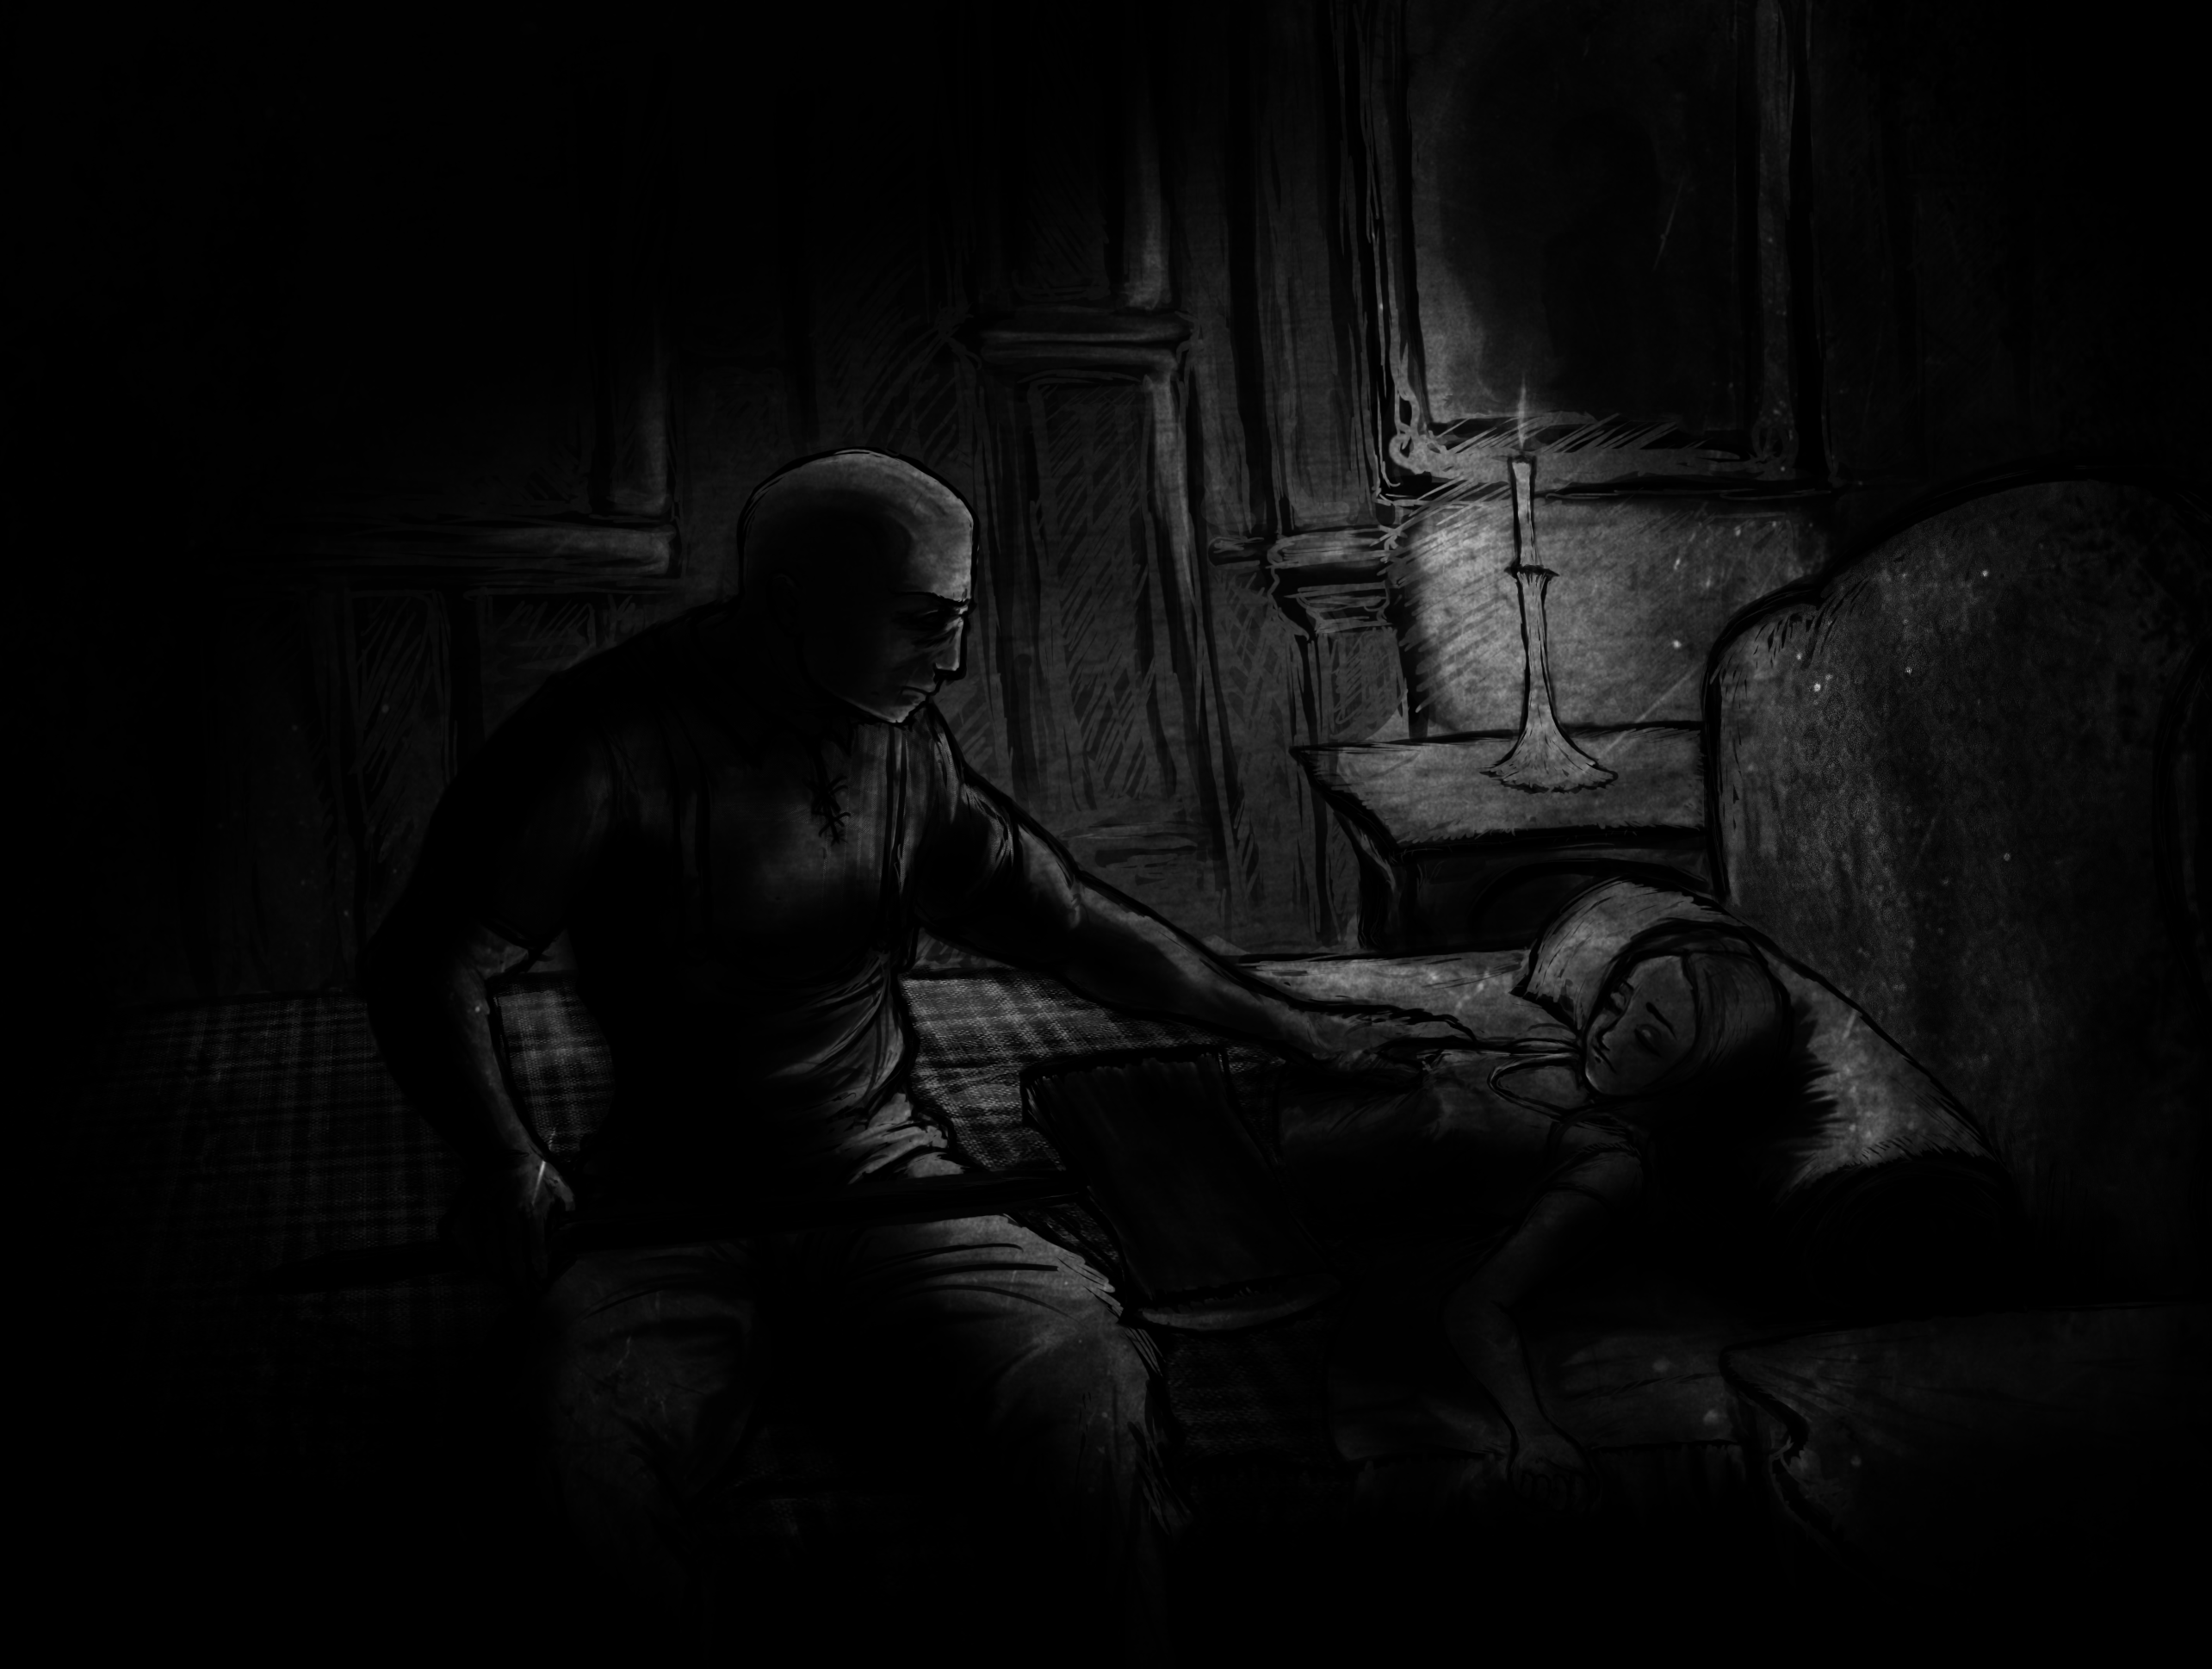
\includegraphics[width=\columnwidth]{lumberjack10}
\end{figure} 

    \paragraph{Ability Scores} Any +2.
    \paragraph{Senses} Nothing special.
    \paragraph{Resistances} Nothing. 
    \paragraph{Weaknesses} Nothing.
    
    \paragraph{Ingenuity} Most characters get a choice of one Primary Attribute in addition to the one granted from their class choice. Instead, the Human character gets to pick two (for a total of three). 
    
    \paragraph{Regional Background} More so than any other Race, Humans are defined more by their homeland and social class than as a Human. 



\section{Minotaur}

Minotaurs are terrible beastmen whose vicious charges on the battlefield have been known to haunt the nightmares of many a fallen and crippled Knight. Despite being monsters, they are a conflicted race. Minotaurs cannot reproduce with their own race for every Minotaur is male, thus they can only spread the seed of their race by polluting the wombs of Human women. In ages past this was primarily done in violent rites of blood sacrifice but this culture has almost died out. This all in all has led to their rarity in Haeckel. Adding to these problems their bovine mouths make it very difficult for them to communicate with the other races. But most tragic fact though is that despite their appearance, on the inside Minotaur's heart and soul shines with an inner light.

The two largest societies of Minotaurs exist in Abyssimiar and Ubris Furor, though there are known to be Minotaurs affected by the Phex that still live in the Old Kingdom of Avalonia. 
 
\begin{figure}[h]
\includegraphics[width=\columnwidth]{Minotaur_sketch}
\end{figure}    
    \paragraph{Ability Scores} +2 STR, +2 WIS, -2 DEX, -2 CHA.
    \paragraph{Senses} 
    \paragraph{Resistances} 
    \paragraph{Weaknesses} 
    
    \paragraph{Alignment} Always Good. 
    \paragraph{Temper} 

\section{Tzuchi}
    A mysterious and foreign race of Snakemen native to the Southern Continent. They are exceedingly rare to see in the fallen Imperial provinces of Haeckel. The Tzuchi are cold blooded sociopaths that are unable to emphathise with warm blooded creatures. In their own homeland they are at the core of the Theocratic religious caste there. Tzuchi whom are on Haeckel are usually on trade expeditions or as part of political envoys. Behind the scenes however Tzuchi aim to covertly infiltrate and dominate the criminal underworld of Haeckel. 
    
    \begin{figure}[h]
\includegraphics[width=\columnwidth]{incubi-celesti}
\end{figure}
    \paragraph{Ability Scores} +2 INT, +2 CON, -2 STR
    \paragraph{Senses} Smell Blood 30ft, Smell Fear 30ft.  
    \paragraph{Resistances} Poison.
    \paragraph{Weaknesses} Holy Weapons. 
    
    \paragraph{Alignment} Always Evil. 
    
    \paragraph{Venomous Bite} The bite of a Tzuchi causes delirious hallucinations in the affected victim. It is said that they see mad visions of a Snake God that torments their nightmares for weeks on end. 
    \paragraph{Sociopathy} Tzuchi are virtually incapable of discerning the emotions or empathising with warm blooded creatures. Any attempt to sense this will fail or worse end with horrific failure.
    \paragraph{Order of the Faith} Tzuchi's theocratic life imposes severe limitations on the behaviour of a Tzuchi. 
    
    The Tzuchi Tribune aim to significantly improve Human-Tzuchi relations and thus enforce that Tzuchi be honest in all their dealings and do what it takes to promote this cause. 
    
    A Tzuchi who is caught being dishonest is most likely going to be eaten by his fellows; thus in any deception it is highly suggested that Tzuchi displace responsibility of conspiracies to others, and to make sure there is always a fall guy as well as any necessary cover stories.
    
    A Tzuchi who fails in these duties is seen as incompetent and thus unworthy to live. Social Darwinism is the status quo in the vicious and cutt-throat competitive Tzuchi Society.  
    \paragraph{Hidden Agenda} Whether for real or imagined reasons, nobody trusts a Tzuchi. 
    
\section{Wood Elf} Wood Elves have had perhaps the most tragic and turbulent histories in Haeckel. At their height they dominated the continent and were seen almost as a master race. The legends speak of the Wood Elves having direction connections with the deities before the Dread Gates existed. 1300 Years ago Humans migrated onto the continent from a faraway land and displaced the status quo. At their lowest the Wood Elves were sold as prized slaves. Their holding onto paganic Old Ways has led them to be scapegoated in certain regions. In others they are held with high regard. 

In regions where there is deep seated discrimination and racism towards the Wood Elves they have organised into guerillas and waged 100 year wars against the Tyrants. Rob merchant caravans, plunder and burn villages, and kill. Instead of finding a peaceful solution, many humans send troops to fight them. In most cases the Tyrant will realise the economic cost imposed upon them for carrying out their hatred and call for peace. Armed rebellion, resistance, and assassination of Human leaders is considered a morally acceptable position of Elves in troubles. Wood Elves find the Human notion of the Divine Right of Kings amusing – whereas this idea is deeply ingrained in most Human cultures. 

Their mobility, sword styles, and ability to disengage combat much more safely than other races makes them some of the best skirmishers in the world. From the tactical situations, to social situations to character development, Wood Elves will have a unique look and feel in real gameplay terms.

\paragraph{Ability Scores} +2 DEX, +2 WIS.
\paragraph{Senses} Twilight Vision, Farsight
\paragraph{Resistances} 
\paragraph{Weaknesses} Iron. 

\paragraph{No Teamwork} Elves do not gain bonuses from flanking, nor can they be flanked.

\paragraph{Martial Arts} Elves do not fight in regimented formations. They require much more space due to the elegant moves of their various fighting styles. Thus for the purposes of combat they count as requiring 10ft by 10ft.  

\begin{framed}\centering
It is intended that Elves whom live long enough eventually become master duelists who are unrivaled in martial prowess. While their Martial Arts trait may not seem like much, this is actually a pretty significant disadvantage in the gameplay of Haeckel RPG. This disadvantage is balanced out by the fact they have no penalty to ability scores and will have the opportunity to gain some of the best combat feats available to any race.   
\end{framed}

\end{multicols}

